\section{Method}
%-------------------------------------------------------------------------------------------------------------

% Harware used
% EEG
\textcolor{violet}{A \href{https://docs.openbci.com/Ganglion/GanglionLanding/}{Ganglion Board} was used to record the EEG signals and sending it to a PC for processing using a \href{https://shop.openbci.com/products/ganglion-dongle}{Ganglion Dongle}.}
\textcolor{violet}{The EEG electrodes used were the OpenBCI \href{https://shop.openbci.com/products/openbci-gold-cup-electrodes}{Gold Cup Electrodes}. The EEG electrodes were first coated with Weaver and Company \href{https://www.weaverandcompany.com/products/ten20/}{Ten20 Conductive Paste} and then attached to the subject using \href{https://www.apotekhjartat.se/product/hjartats-kirurgtejp-brun-25-cm-x-91-m/}{surgical tape}.}
\textcolor{teal}{The \href{https://brainflow.readthedocs.io/en/stable/index.html}{Brainflow API} was used to receive and timestamp the EEG signals recorded on the \href{https://docs.openbci.com/Ganglion/GanglionLanding/}{Ganglion Board} transmitted over bluetooth.}

% EMG
\textcolor{violet}{Two \href{https://wiki.seeedstudio.com/Grove-EMG_Detector/}{Grove EMG Detectors} were used for recording the EMG signals.}
\textcolor{violet}{The EMG electrodes used were the 3M \href{https://www.3m.com/3M/en_US/p/d/b00037638/}{Red Dot Monitoring Electrode}.}
\textcolor{teal}{The \href{https://www.ni.com/en/shop/engineering-education/portable-student-devices/mydaq/what-is-mydaq.html}{NI myDAQ} was used to receive and timestamp the EMG signals recorded from the \href{https://wiki.seeedstudio.com/Grove-EMG_Detector/}{Grove EMG Detector}.}

% Software
\textcolor{teal}{The \href{https://github.com/ROBOTIS-GIT/turtlebot3}{Turtlebot3}, simulated in \href{https://gazebosim.org/home}{Gazebo}, received commands through a \href{https://docs.ros.org/en/humble/index.html}{ROS2 humble} interface in \href{https://se.mathworks.com/products/matlab.html}{Matlab} running on Windows 11.}
\textcolor{olive}{The \href{https://docs.openbci.com/Software/OpenBCISoftware/GUIDocs/}{OpenBCI GUI} software was used to evaluate EEG electrode contact by impedance test.}
\textcolor{violet}{\href{https://se.mathworks.com/products/matlab.html}{Matlab R2023b} was used for handling all the data once it was on the PC and for all signal processing.}

% Github
\textcolor{violet}{All code used for this study can be found on \href{https://github.com/ELA411}{Github} and is open source.}

%-------------------------------------------------------------------------------------------------------------

\subsection{Experimental Setup and Signal Acquisition}
% 2 reference electrodes needed for the impedance check to pass, one on each ear
% EEG electrodes
\textcolor{violet}{Four EEG electrodes, resulting in four channels, were used and placed over the motorcortex, adapting the $10-20$ system to four electrodes. The specific locations were $\text{C}1$ (channel 3), $\text{CP}1$ (channel 4), $\text{C}5$ (channel 1), $\text{CP}5$ (channel 2). Two reference electrodes were used and was placed on the left ($\text{A}1$) and right ($\text{A}2$) earlobe.}
\textcolor{violet}{See Fig.\:\ref{fig:eeg_left} and Fig.\:\ref{fig:eeg_right} for all EEG electrode locations. The electrodes were coated in Weaver and Company \href{https://www.weaverandcompany.com/products/ten20/}{Ten20 Conductive Paste} before being attached with \href{https://www.apotekhjartat.se/product/hjartats-kirurgtejp-brun-25-cm-x-91-m/}{surgical tape}.}
\textcolor{olive}{Before sampling, to ensure the electrodes had good contact, an impedance test was done in the \href{https://docs.openbci.com/Software/OpenBCISoftware/GUIDocs/}{OpenBCI GUI}. Each electrode needed a value below $20\:\text{k}\Omega$ to be valid.} 
\textcolor{violet}{The EEG signal was sampled at $200\:\text{Hz}$.}

% EEG task
\textcolor{violet}{The drive forward command was controlled by MI of closing the right hand. The do not drive command was controlled by the resting state (no MI). See Table.\:\ref{tab:eeg_commands} for the classes of the different EEG commands.}

% TABLE EEG COMMANDS
\begin{table}
	\centering
	\begin{tabular}{|l|l|l|l|l|}
		\hline
		Command                               & Class \\
		\hline
		Do not drive (resting, no MI)         & 0     \\
		Drive forward (MI closing right hand) & 1     \\
		\hline
	\end{tabular}
	\caption{All EEG commands and their respective class.}
	\label{tab:eeg_commands}
\end{table}

% FIGURE EEG LOCATIONS
\begin{figure}
	\centering
	\begin{subfigure}[b]{0.45\columnwidth}
		\centering
		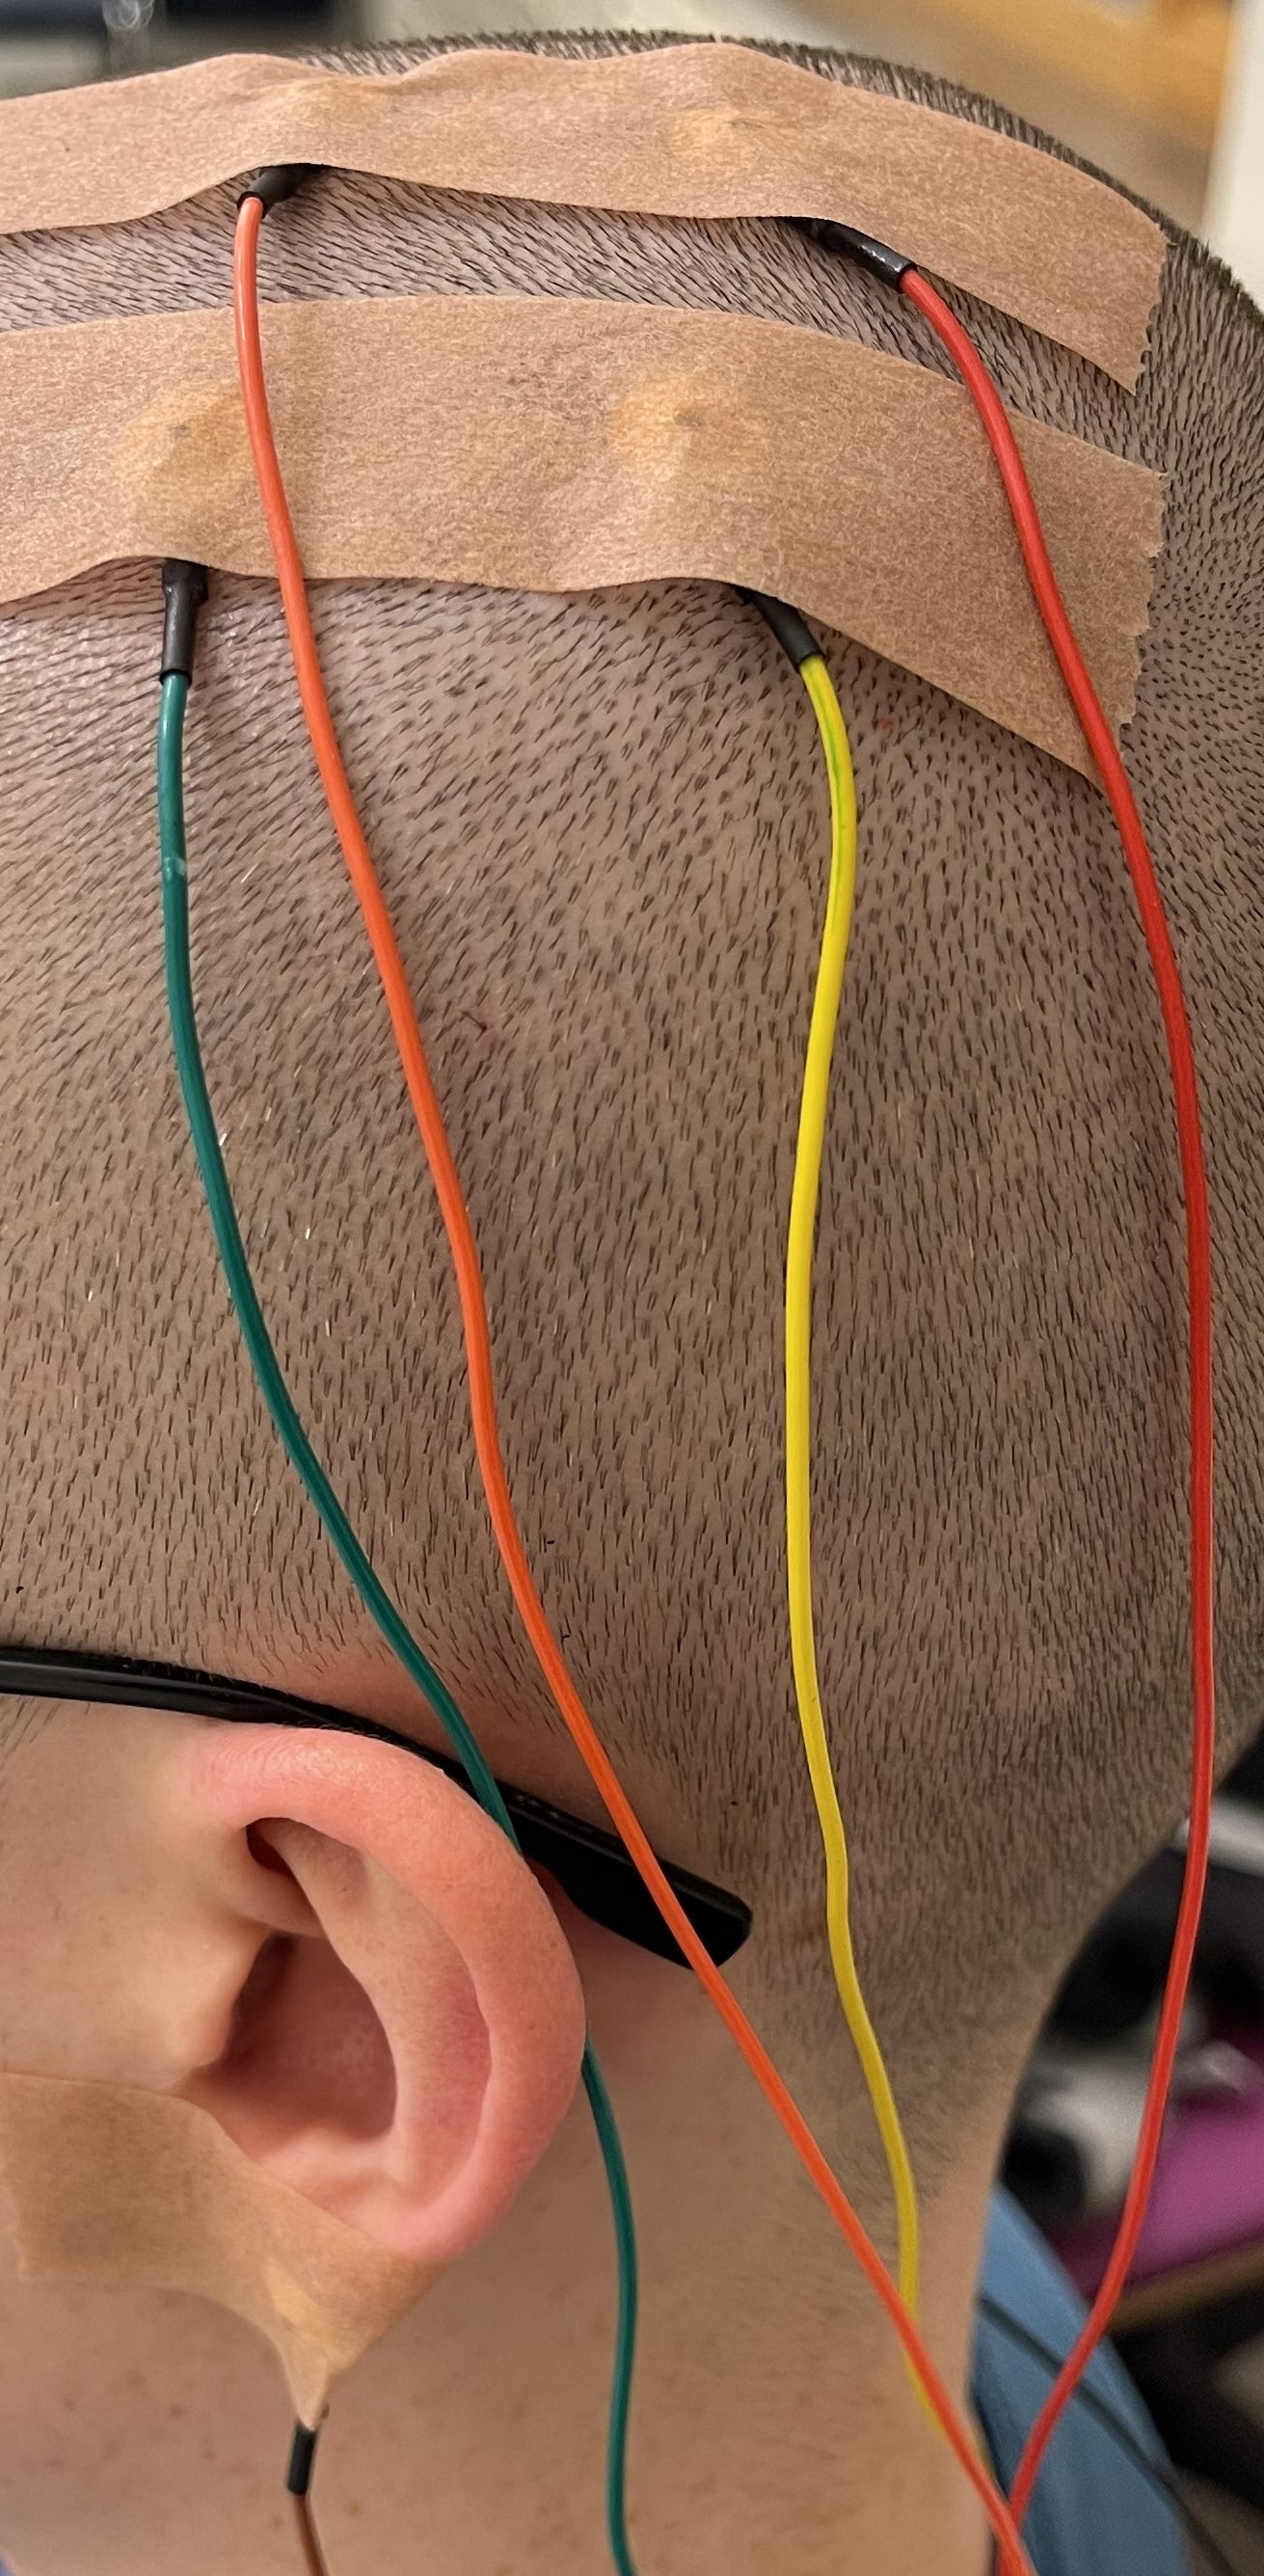
\includegraphics[height=3cm]{figures/eeg_left.jpg}
		\caption{The reference electrode on the left earlobe, $\text{A}1$ (brown). Channel $1$ on $\text{C}5$ (green), channel $2$ on $\text{CP}5$ (yellow), channel $3$ on $\text{C}1$ (orange) and channel $4$ on $\text{CP}1$ (red).}
		\label{fig:eeg_left}
	\end{subfigure}
    \begin{subfigure}[b]{0.45\columnwidth}
		\centering
		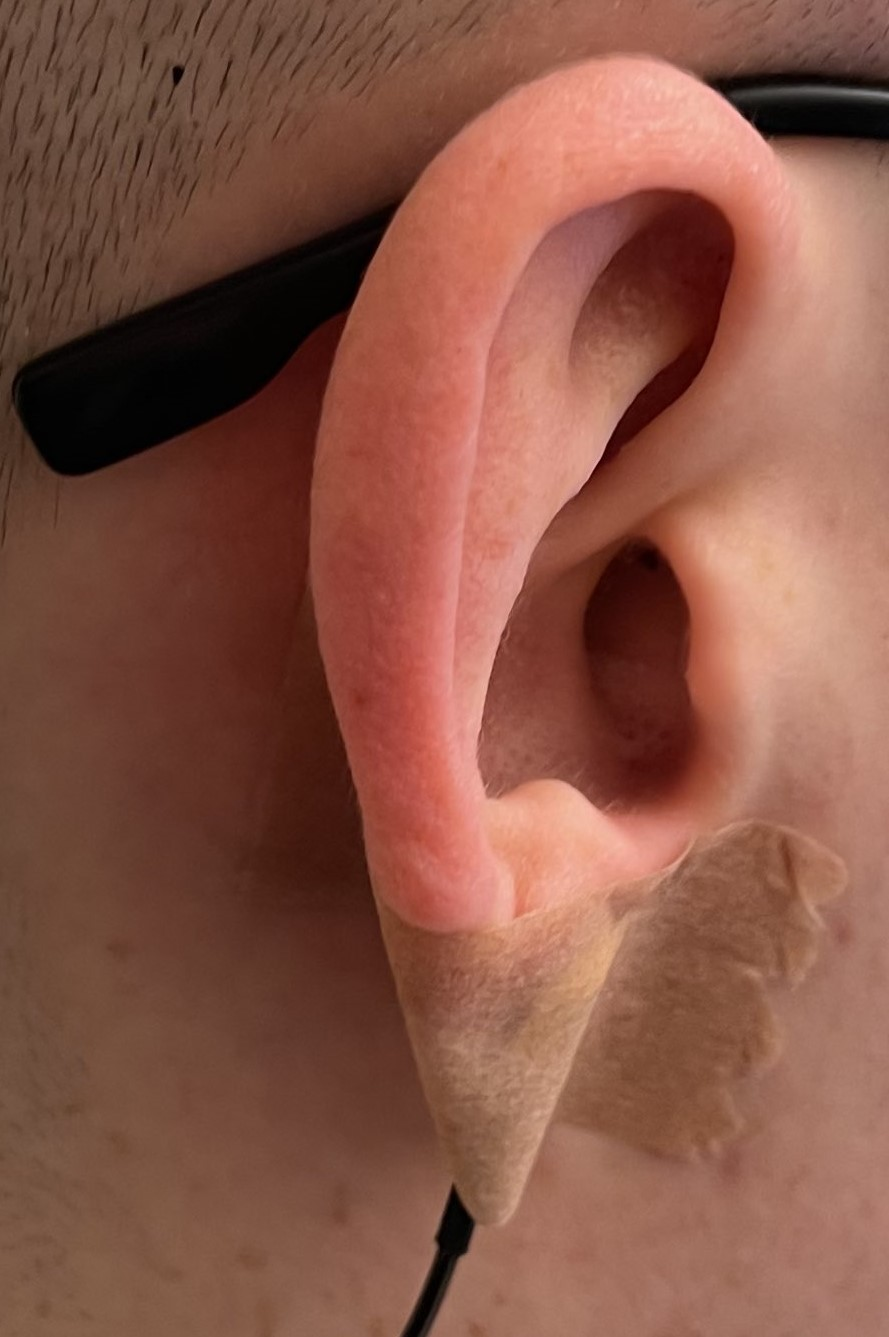
\includegraphics[height=3cm]{figures/eeg_right.jpg}
		\caption{The reference electrode on the right earlobe, $\text{A}2$ (black).}
		\label{fig:eeg_right}
	\end{subfigure}
    \hfill
	\caption{All EEG electrode positions.}
	\label{fig:eeg_electrodes}
\end{figure}

% EMG electrodes
\textcolor{violet}{Four EMG bipolar electrodes were used, resulting in two channels, placed on the left arm. One set was placed longitudinally (channel $1$) and the other transversely (channel $2$) over the left forearm muscles flexor carpi radialis, palmaris longus and flexor carpi ulinaris. Two reference electrodes, one for each channel, were placed on the elbow of the left arm, specifically the olecranon and the lateral epicondyle. The interelectrode distance was $4\:\text{cm}$. See Fig.\:\ref{fig:emg_electrodes} and Fig.\:\ref{fig:emg_reference} for all EMG electrode locations. Before electrodes were placed, the skin was cleaned with alcohol and any hair was removed to improve signal quality\:\cite{khanSelectionFeaturesClassifiers2020}. The EMG signal was sampled at $1000\:\text{Hz}$.}

% EMG task
\textcolor{violet}{The turn left command was controlled by left wrist extension. The turn right command was controlled by left wrist flexion. No turning occurs when in resting state. See Table.\:\ref{tab:emg_commands} for the classes of the different EMG commands.}
% TABLE EMG COMMANDS
\begin{table}
	\centering
	\begin{tabular}{|l|l|l|l|l|}
		\hline
		Command                                                  & Class \\
		\hline
		No turning (resting, no left wrist extension or flexion) & 0     \\
		Turn left (left wrist extension)                         & 1     \\
		Turn right (left wrist flexion)                          & 2     \\
		\hline
	\end{tabular}
	\caption{All EMG commands and their respective class.}
	\label{tab:emg_commands}
\end{table}

% FIGURE EMG ELECTRODE POSITIONS
\begin{figure}
	\centering
	\begin{subfigure}[b]{0.45\columnwidth}
		\centering
		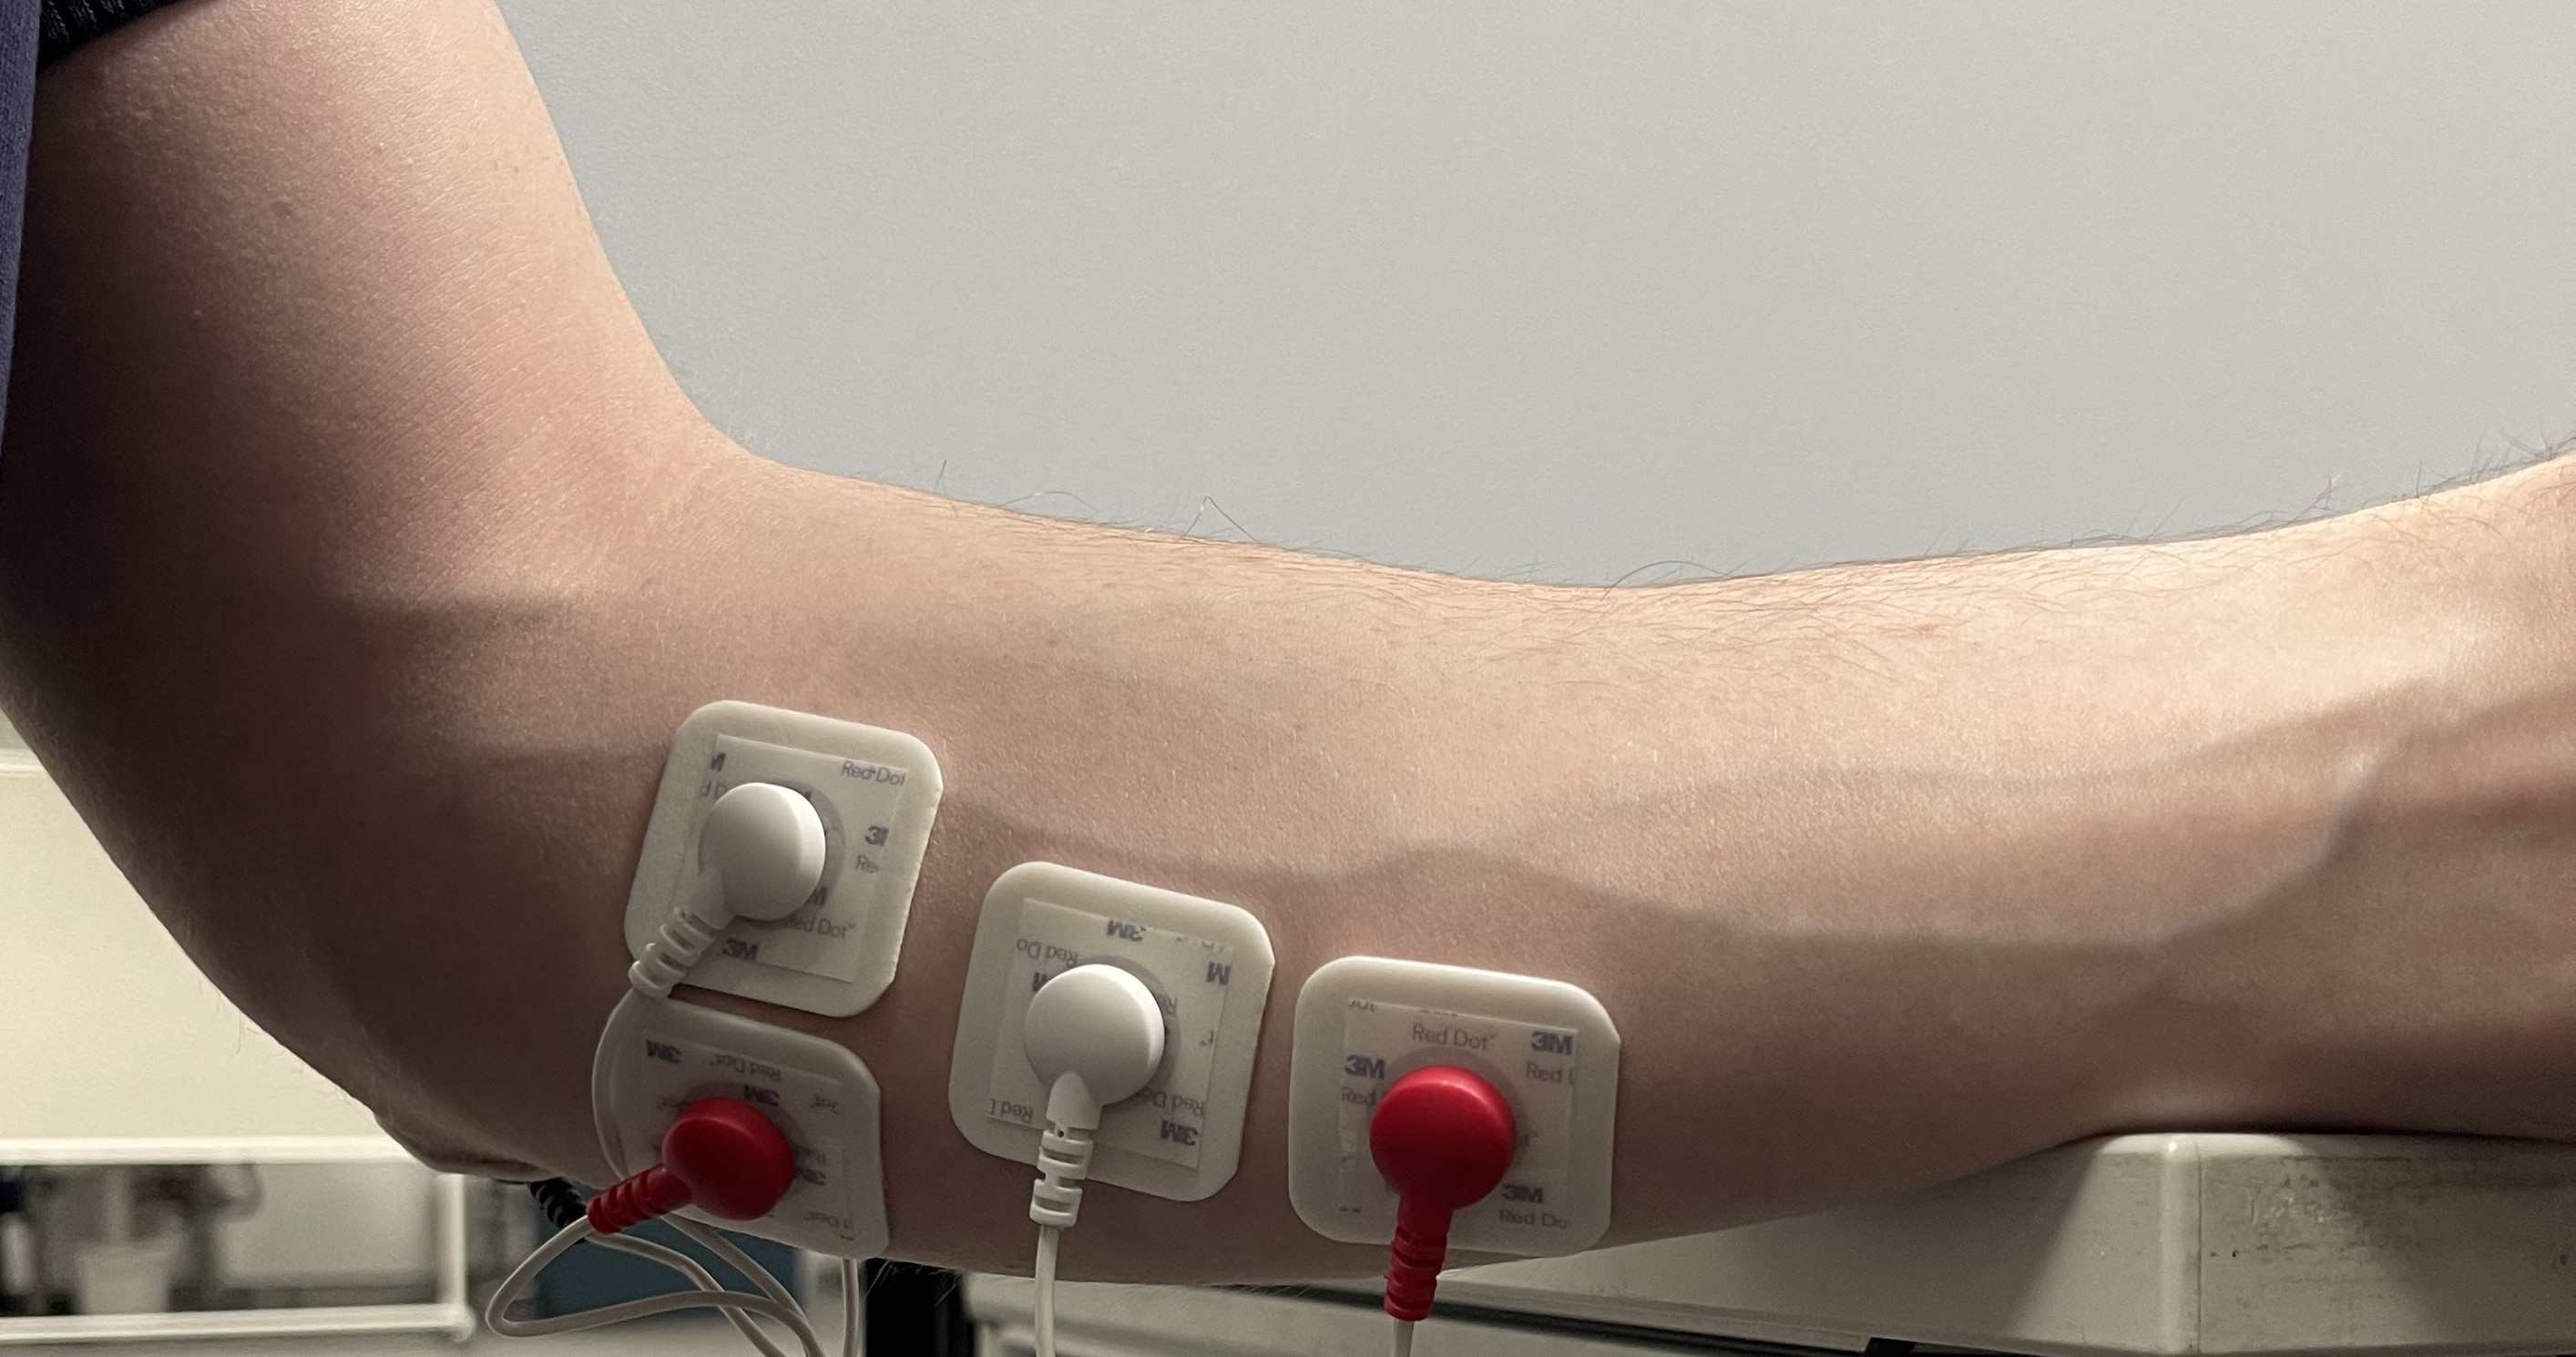
\includegraphics[width=\columnwidth]{figures/emg_electrodes.jpg}
		\caption{The EMG bipolar electrode locations, one set placed longitudinally (channel $1$) and the other transversely (channel $2$) over the flexor carpi radialis, palmaris longus and flexor carpi ulinaris muscles of the left forearm.}
		\label{fig:emg_electrodes}
	\end{subfigure}
	\begin{subfigure}[b]{0.45\columnwidth}
		\centering
		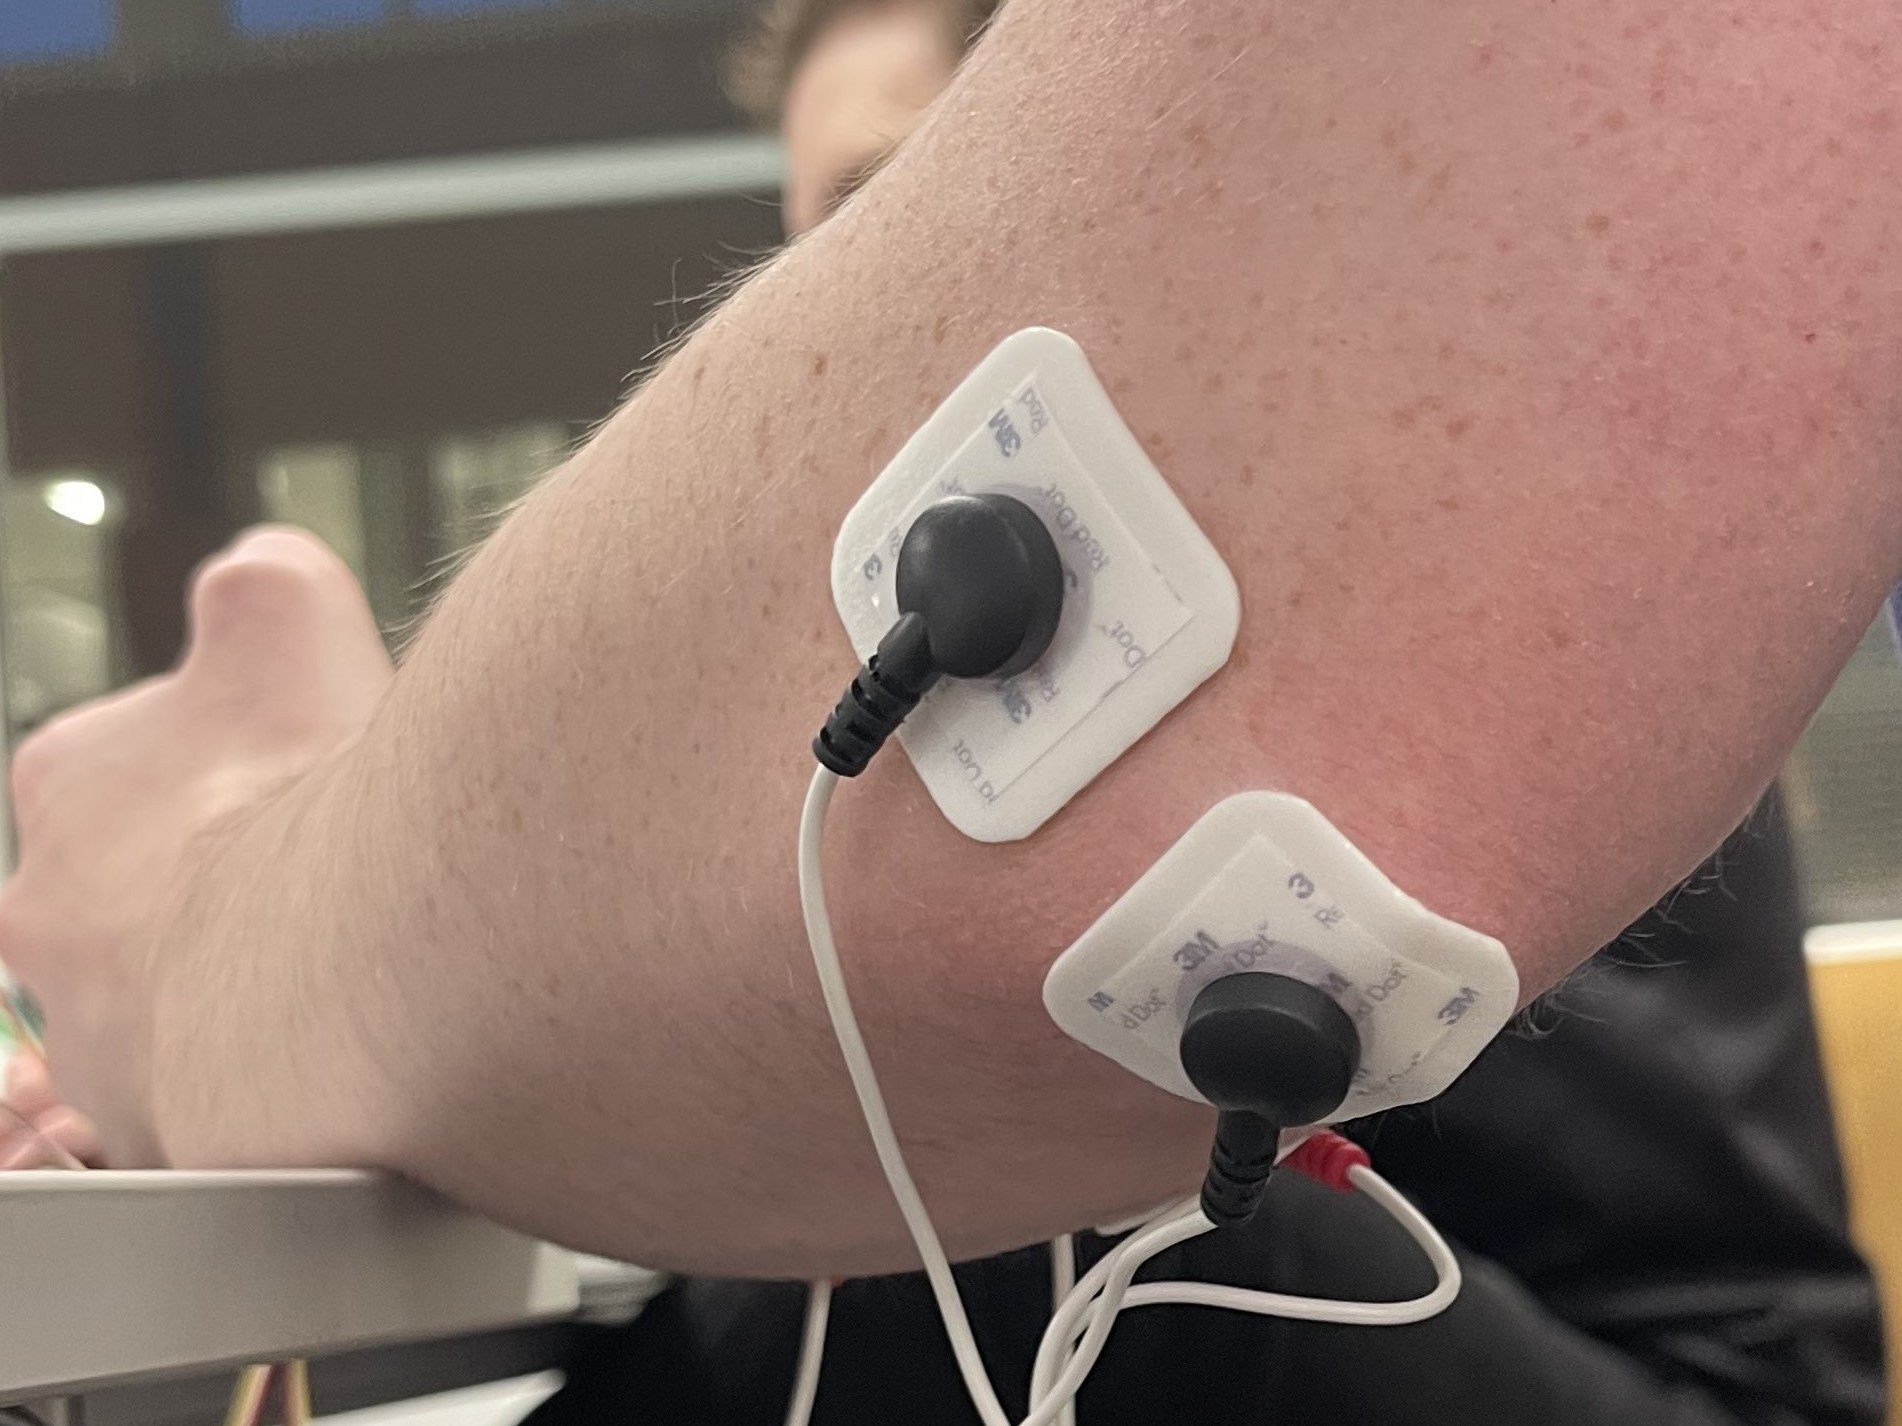
\includegraphics[width=\columnwidth]{figures/emg_reference.jpg}
		\caption{The EMG reference electrodes placed on the olecranon and the lateral epicondyle of the left arm.}
		\label{fig:emg_reference}
	\end{subfigure}
    \hfill
	\caption{All EMG electrode positions.}
	\label{fig:emg_positions}
\end{figure}

% Dataset
\textcolor{violet}{Six different models were created, three EEG classifiers and three EMG classifiers, one EEG/EMG pair for each subject. Each subject created one EEG and one EMG dataset to train and validate their own models on. The datasets consisted of:
	\begin{itemize}
		\item EEG dataset
		      \begin{itemize}
			      \item $50$ repetitions of MI closing right hand for $4\:\text{s}$
			      \item $4\:\text{s}$ pause between repetitions
		      \end{itemize}
		\item EMG dataset
		      \begin{itemize}
			      \item $30$ repetitions of left wrist extension, held for $4\:\text{s}$
			      \item $30$ repetitions of left wrist flexion, held for $4\:\text{s}$
			      \item $4\:\text{s}$ pause between repetitions
		      \end{itemize}
	\end{itemize}}
\textcolor{violet}{The creation of each EMG dataset followed a schedule where first one repetition of left wrist extension was done, then one repetition of left wrist flexion with pause in between and then looping back until $30$ receptions of each movement had been done. Then after the EMG movements were done the EEG MI were recorded, this followed the schedule of: one repetition of MI closing right hand, pause and then looping back until $50$ repetitions had been completed. Example runs of the dataset schedules can be seen in Fig.\:\ref{fig:eeg_task} and Fig.\:\ref{fig:emg_task}.}
\textcolor{violet}{All EMG movements were performed with full force.}
\textcolor{violet}{The subject was sitting with the left arm at $90\degree\:$ angle, resting on a table when the dataset was created as well as for online testing of the system. See Fig.\:\ref{fig:emg_positions} for the left arm position.}
\textcolor{olive}{The subjects right arm was relaxed and hanging straight down while performing MI.}
\textcolor{olive}{One EEG test set was created from actual right hand closing motions, and another from only MI. Its purpose was to verify that MI actually can be identified with the equipment used by detecting a real motion and an imagery one.}
\textcolor{violet}{See Discussion\:\ref{section:discussion} for comments on this test EEG dataset with actual right hand closing motion.}
\textcolor{violet}{The datasets and the EEG and EMG commands were labeled using a script which switched the label it added to the corresponding samples according to the schedules presented above, see Fig.\:\ref{fig:task_schedule}.}
\textcolor{violet}{The average number of EEG samples in each EEG dataset was $80258 \pm 845$, and the average number of EMG samples in each EMG dataset was $421566 \pm 101310$.}
\textcolor{violet}{The average class distribution in each EEG dataset can be seen in Table.\:\ref{tab:eeg_class_distribution} and for the EMG datasets can be seen in Table.\:\ref{tab:emg_class_distribution}.}
\textcolor{violet}{The duration of a EEG data collection session was $400\:\text{s}$, and for EMG it was $480\:\text{s}$.}
\textcolor{violet}{Table.\:\ref{tab:eeg_dataset} shows the impedance of all the EEG electrodes for each of the EEG datasets of each subject. Because of the impedance of channel $3$ (see Table.\:\ref{tab:eeg_dataset}) for each subject, it had to be excluded.}
\textcolor{violet}{The subjects consisted of the authors of the paper, three Scandinavian men of Swedish nationality with no prior BCI experience, ages $22$, $23$, $23$.}

% Class distribution
\begin{table}[ht]
    \centering
    \begin{tabular}{c|c}
         class 0 (\%)           & class 1 (\%)             \\ \hline
         $50.16 \pm 0.30$       & $49.84 \pm 0.30$
    \end{tabular}
    \caption{Average class distribution in the EEG datasets.}
    \label{tab:eeg_class_distribution}
\end{table}
\begin{table}[ht]
    \centering
    \begin{tabular}{c|c|c}
         class 0 (\%)           & class 1 (\%)          & class 2 (\%)            \\ \hline
         $50.15 \pm 0.23$       & $25.00 \pm 0.14$      & $24.84 \pm 0.34$
    \end{tabular}
    \caption{Average class distribution in the EMG datasets.}
    \label{tab:emg_class_distribution}
\end{table}

% IMPEDANCE
\begin{table}[ht]
	\centering{
		\resizebox{\columnwidth}{!}{\noindent\begin{tabular}{|l|l|l|l|l|l|}
			\hline
		  Metric (Subject)	            & channel $1$              & channel $2$               & channel $3$                   & channel $4$               & combined refs                 \\ \hline
			Impedance ($\text{s}_1$)      & $13.0\:\text{k}\Omega$   & $17.5\:\text{k}\Omega$    & $10737.0\:\text{k}\Omega$     & $22.5\:\text{k}\Omega$    & $8.0\:\text{k}\Omega$         \\ \hline
			Position ($\text{s}_1$)       & $\text{C}5$              & $\text{CP}5$              & $\text{C}1$                   & $\text{CP}1$              & $\text{A}1$ \& $\text{A}2$    \\ \hline
            Impedance ($\text{s}_2$)      & $14.5\:\text{k}\Omega$   & $11.5\:\text{k}\Omega$    & $10737.0\:\text{k}\Omega$     & $14.5\:\text{k}\Omega$    & $6.0\:\text{k}\Omega$         \\ \hline
			Position ($\text{s}_2$)       & $\text{C}5$              & $\text{CP}5$              & $\text{C}1$                   & $\text{CP}1$              & $\text{A}1$ \& $\text{A}2$    \\ \hline
            Impedance ($\text{s}_3$)      & $12.5\:\text{k}\Omega$   & $10.5\:\text{k}\Omega$    & $10737.0\:\text{k}\Omega$     & $16.5\:\text{k}\Omega$    & $10.5\:\text{k}\Omega$        \\ \hline
			Position ($\text{s}_3$)       & $\text{C}5$              & $\text{CP}5$              & $\text{C}1$                   & $\text{CP}1$              & $\text{A}1$ \& $\text{A}2$    \\ \hline
		\end{tabular}}
	}
	\caption{EEG electrode impedance and electrode position for each channel, for all EEG datasets.}
	\label{tab:eeg_dataset}
\end{table}


% FIGURE TASK SCHEDULE
\begin{figure}
	\centering
    \begin{subfigure}[b]{0.45\columnwidth}
		\centering
		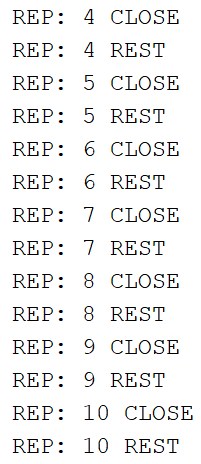
\includegraphics[height=5cm]{figures/eeg_task.png}
		\caption{Example part of the EEG task procedure followed during dataset creation.}
		\label{fig:eeg_task}
	\end{subfigure}	
    \begin{subfigure}[b]{0.45\columnwidth}
		\centering
		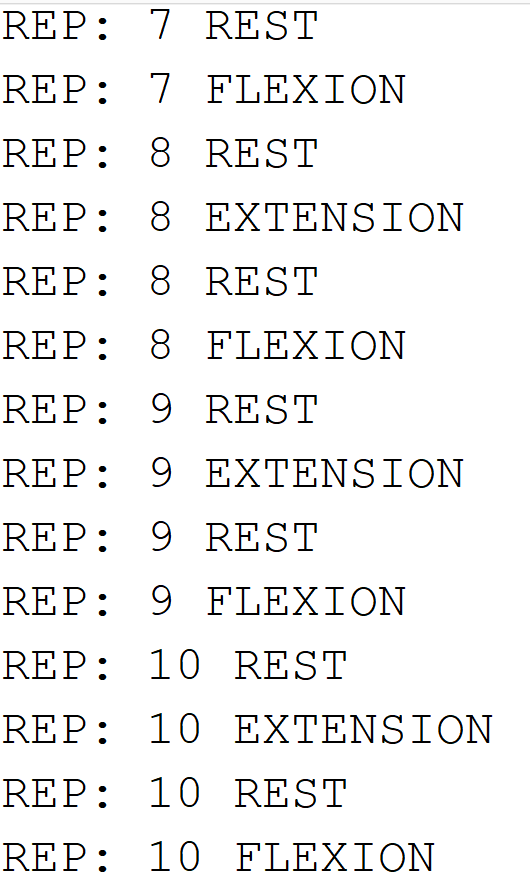
\includegraphics[height=5cm]{figures/emg_task.png}
		\caption{Example part of the EMG task procedure followed during dataset creation.}
		\label{fig:emg_task}
	\end{subfigure}
	\hfill
	\caption{Task schedule for EEG and EMG.}
	\label{fig:task_schedule}
\end{figure}


% Time stamp
\textcolor{violet}{The EEG data was timestamped by the Brainflow API when it was received on the PC.}
\textcolor{teal}{The EMG data was timestamped by the NI myDAQ.}
% Streaming
\textcolor{teal}{The \href{https://docs.openbci.com/Ganglion/GanglionLanding/}{Ganglion Board} records the EEG signals and transmits them to a PC over bluetooth with a frequency of $100\:\text{Hz}$, however two data samples are sent as one package, resulting in a theoretical frequency of $200\:\text{Hz}$\:\cite{OpenBCI2023}. The \href{https://brainflow.readthedocs.io/en/stable/index.html}{Brainflow API} was used to enable the streaming of the EEG data.}
\textcolor{teal}{The EMG signals were recorded by a \href{https://www.ni.com/en/shop/engineering-education/portable-student-devices/mydaq/what-is-mydaq.html}{NI myDAQ} which converts the analog input of the \href{https://wiki.seeedstudio.com/Grove-EMG_Detector/}{Grove EMG Detector} with a frequency of $1000\:\text{Hz}$.}

%-------------------------------------------------------------------------------------------------------------

\subsection{Signal Handling}
% Storing
\textcolor{violet}{The received signals were both stored for offline processing and analysis as well as being processed online.}

% Data lost
\textcolor{violet}{The number of lost EMG packages was calculated by incrementing the number of lost packages whenever a successive package ID was not the previous package ID plus one modulo $1000$. The modulo $1000$ is a result of the EMG package IDs looping from $0$ to $1000$.}
\textcolor{violet}{The number of lost EEG packages was calculated in the same way as the EMG but it needed to account for duplicate IDs (a result of sending two samples each time) as well as package ID going from $100$ to $200$ rather than $0$ to $1000$. The reader is directed to the code available on \href{https://github.com/ELA411}{Github} for a complete understanding of the EEG data lost implementation.}
% Data lost online
\textcolor{teal}{The EMG data collected online does not contain package IDs, therefor, to calculate the number of EMG packages lost, the time differences between consecutive samples was taken and then compared to a threshold of $0.0015$ seconds. Because of processing times in matlab, a $0.0005$ seconds buffer is taken into account.}

% Signal quality
\textcolor{teal}{The signal quality was evaluated by extracting the signal-to-noise ratio (SNR), signal-to-noise and distortion ratio (SINAD), and total harmonic distortion (THD) from the recorded signal. Signal quality was also evaluated by comparing the actual sample rate ($f_{sampling}$) with the sample rate recorded in \href{https://se.mathworks.com/products/matlab.html}{Matlab}, $f_{recorded}$, see\:\eqref{eq:freq_recorded}.}
\textcolor{teal}{\begin{dmath}
		\label{eq:freq_recorded}
		f_{recorded} = \frac{1}{T}
	\end{dmath}}
% Period
\textcolor{teal}{The period for the EEG and EMG was calculated by taking the time differences between consecutive samples, and taking the mean value to get the average period between samples, $T$, }\textcolor{violet}{see\:\eqref{eq:period}.
	\begin{dmath}
		\label{eq:period}
		T = \frac{\sum_{n = 2}^{m} t_n-t_{n-1}}{m}
	\end{dmath}
	where $t_n$ is the timestamp of the current package, $t_{n-1}$ is the timestamp of the previous package and $m$ is the total number of packages.}
\textcolor{violet}{The data lost and data quality of each dataset is shown in Table.\:\ref{tab:lost_quality}. The $2$ samples being lost for EEG is the result of the \href{https://docs.openbci.com/Ganglion/GanglionLanding/}{Ganglion Board} transmission protocol always losing the two samples in package $199$ during the first cycle.}
% TABLE DATA LOST AND QUALITY
\begin{table}[ht]
	\centering
	\begin{tabular}{|l|l|l|l|l|}
			\hline
			Metric                                & $\text{s}_1$      & $\text{s}_2$      &   $\text{s}_3$            \\
			\hline
			Data lost EEG                         & $2$               & $2$               & $2$                       \\
			Data lost EMG                         & $0$               & $0$               & $0$                       \\
			EEG $f_{recorded}$ ($\text{Hz}$)      & $199.01$          & $199.01$          & $199.02$                  \\
            EMG $f_{recorded}$ ($\text{Hz}$)      & $1000.00$         & $1000.00$         & $1000.00$                 \\
            EEG channel 1 SNR ($\text{dB}$)       & $-4.11$           & $-4.75$           & $4.94$                    \\
            EEG channel 1 SINAD                   & $-\infty$         & $-\infty$         & $-2.10$                   \\
            EEG channel 1 THD                     & $-4.11$           & $-4.75$           & $4.93$                    \\
            EEG channel 2 SNR ($\text{dB}$)       & $0.77$            & $-0.12$           & $2.33$                    \\
            EEG channel 2 SINAD                   & $-\infty$         & $-1.20$           & $-2.14$                   \\
            EEG channel 2 THD                     & $0.77$            & $-0.12$           & $2.32$                    \\
            EEG channel 3 SNR ($\text{dB}$)       & $1.19$            & $-4.46$           & $1.84$                    \\
            EEG channel 3 SINAD                   & $-\infty$         & $-\infty$         & $-\infty$                 \\
            EEG channel 3 THD                     & $1.19$            & $-4.46$           & $1.84$                    \\
            EEG channel 4 SNR ($\text{dB}$)       & $1.00$            & $-2.50$           & $3.67$                    \\
            EEG channel 4 SINAD                   & $-\infty$         & $-2.52$           & $-2.09$                   \\
            EEG channel 4 THD                     & $1.00$            & $-2.50$           & $3.67$                    \\
            EMG channel 1 SNR ($\text{dB}$)       & $-16.06$          & $-0.25$           & $-18.22$                  \\
            EMG channel 1 SINAD                   & $-3.09$           & $-57.96$          & $3.32$                    \\
            EMG channel 1 THD                     & $-16.10$          & $-0.25$           & $-18.36$                  \\
            EMG channel 2 SNR ($\text{dB}$)       & $-12.24$          & $-1.79$           & $0.85$                    \\
            EMG channel 2 SINAD                   & $-43.24$          & $-51.96$          & $-55.54$                  \\ 
            EMG channel 2 THD                     & $-12.24$          & $-1.79$           & $0.85$                    \\
			\hline
		\end{tabular}
	\caption{The data lost and data quality for each dataset.}
	\label{tab:lost_quality}
\end{table}

% Visualize signal
\textcolor{violet}{The EEG and EMG signals were plotted and displayed in \href{https://se.mathworks.com/products/matlab.html}{Matlab}.}

%-------------------------------------------------------------------------------------------------------------

\subsection{Preprocessing}
% Filtering
\textcolor{violet}{The EEG signal was filtered by:
	\begin{itemize}
		\item A $0.1$ to $99\:\text{Hz}$ $4$th order Butterworth bandpass filter to remove DC offset and baseline wandering, as well as adhering to the assumption that the signal fed to the log band power feature extraction has been bandpass filtered, see Introduction\:\ref{section:intro}
		\item Two $4$th order IIR notch filters with quality factor $30$ and $1\:\text{dB}$ passband ripple was applied to remove $50\:\text{Hz}$ power line noise as well as the second harmonic ($100\:\text{Hz}$).
	\end{itemize}}
\textcolor{violet}{The EMG signal was filtered by:
	\begin{itemize}
		\item A $20$ to $499\:\text{Hz}$ $4$th order Butterworth bandpass filter to remove DC offset, baseline wandering and high frequencies
		\item Three $4$th order IIR notch filters with quality factor $30$ and $1\:\text{dB}$ passband ripple was applied to remove $50\:\text{Hz}$ power line noise as well as the second ($100\:\text{Hz}$) and third ($150\:\text{Hz}$) harmonic.
	\end{itemize}}

% CSP
\textcolor{violet}{The W matrix for CSP was created after filtering but was not applied until the feature extraction step when the signal had been segmented. The acquired W matrix from CSP, was only created during offline processing and was then saved for later use in real-time using the \href{https://se.mathworks.com/products/matlab.html}{Matlab} \href{https://se.mathworks.com/help/matlab/ref/save.html}{save} and \href{https://se.mathworks.com/help/matlab/ref/load.html}{load} functions. CSP was implemented with the \href{https://se.mathworks.com/products/matlab.html}{Matlab} toolbox \href{https://se.mathworks.com/matlabcentral/fileexchange/72204-common-spatial-patterns-csp}{Common Spatial Patterns (CSP)}.}

%-------------------------------------------------------------------------------------------------------------

\subsection{Segmentation}
\textcolor{violet}{The EEG signal was segmented into $250\:\text{ms}$ windows with $50\:\text{ms}$ overlap. The EEG window size and overlap was chosen to align with EMG to simplify online implementation.}
\textcolor{violet}{The EMG signal was segmented into $250\:\text{ms}$ windows with $50\:\text{ms}$ overlap.}
\textcolor{violet}{Offline segmentation was implemented using the \href{https://se.mathworks.com/products/matlab.html}{Matlab} function \href{https://se.mathworks.com/help/signal/ref/buffer.html}{buffer}.}

%-------------------------------------------------------------------------------------------------------------

\subsection{Feature Extraction}
% EEG
\textcolor{violet}{The feature extraction methods for the EEG signal was variance of the PSD of the beta band ($\beta = [12,\:30]\:\text{Hz}$) and log band power of the CSP.}
% Beta band variance
\textcolor{violet}{The variance of the PSD of the beta band consisted of calculating the PSD of the window\:\eqref{eq:psd_window}, extracting the beta band ($\beta = [12,\:30]\:\text{Hz}$) frequencies\:\eqref{eq:extract_beta} and calculating the variance\:\eqref{eq:psd_variance}. The PSD was calculated using \href{https://se.mathworks.com/help/signal/ref/pwelch.html}{pwelch} and the variance using \href{https://se.mathworks.com/help/matlab/ref/var.html}{var}.}
\textcolor{violet}{
	\begin{dmath}
		\label{eq:psd_window}
		PSD_{window} = PSD(data_{window})
	\end{dmath}
	\begin{dmath}
		\label{eq:extract_beta}
		PSD_{\beta} = extract\_\beta(PSD_{window})
	\end{dmath}
	\begin{dmath}
		\label{eq:psd_variance}
		PSD_{\beta\_variance} = var(PSD_{\beta})
	\end{dmath}}
% CSP log band power
\textcolor{violet}{The log band power of the CSP consisted of CSP filtering the window\:\eqref{eq:csp} and then taking the log band power of the CSP filtered data\:\eqref{eq:log_power}. Note that\:\eqref{eq:csp} assumes that the input data ($data_{window}$) is in the format of $C \times O$ where $C$ is the channels and $O$ are the observations. The log band power was implemented using the \href{https://se.mathworks.com/products/matlab.html}{Matlab} functions \href{https://se.mathworks.com/help/matlab/ref/log.html}{log} and \href{https://se.mathworks.com/help/signal/ref/bandpower.html}{bandpower}.}
\textcolor{violet}{
	\begin{dmath}
		\label{eq:csp}
		data_{CSP} = W^T \times data_{window}
	\end{dmath}
	\begin{dmath}
		\label{eq:log_power}
		CSP_{log\_band\_power} = log(band\_power(data_{CSP}))
	\end{dmath}
}

% EMG
\textcolor{violet}{The feature extraction method used for the segmented EMG data was TDAR. The TD features extracted were: mean absolute value, waveform length, zero crossing and slope sign change. TDAR was implemented in \href{https://se.mathworks.com/products/matlab.html}{Matlab} using the toolbox \href{https://se.mathworks.com/matlabcentral/fileexchange/71514-emg-feature-extraction-toolbox}{EMG Feature Extraction Toolbox}.}

%-------------------------------------------------------------------------------------------------------------

\subsection{Classifier}
\textcolor{violet}{The classifier used for EEG was RBF SVM, implemented by using \href{https://se.mathworks.com/help/stats/fitcsvm.html}{fitcsvm} with kernel function 'rbf' and the \href{https://se.mathworks.com/help/stats/linearmodel.predict.html}{predict} functions.}
\textcolor{violet}{The classifier used for EMG was LDA, implemented by using \href{https://se.mathworks.com/help/stats/fitcdiscr.html}{fitcdiscr} with discriminant type 'pseudolinear' and the \href{https://se.mathworks.com/help/stats/linearmodel.predict.html}{predict} functions.}
\textcolor{violet}{A trained classifier was saved using the \href{https://se.mathworks.com/products/matlab.html}{Matlab} \href{https://se.mathworks.com/help/matlab/ref/save.html}{save} function and loaded using the \href{https://se.mathworks.com/help/matlab/ref/load.html}{load} function.}
\textcolor{violet}{In order to prevent class imbalance the data was subjected to random oversampling before training the classifiers, using \href{https://se.mathworks.com/matlabcentral/fileexchange/75401-synthetic-minority-over-sampling-technique-smote}{Synthetic Minority Over-sampling Technique (SMOTE)}.}
\textcolor{violet}{The balanced data was split into train test splits, with $80\%$ train split and $20\%$ test split. The train split was used for training the classifiers and permutation test $2$. The test split was used when the classifiers performed predictions, namely confusion matrices, permutation test $1$ and binomial tests.}

% Evaluation of classifier
\textcolor{violet}{The classifiers were evaluated using k-fold cross validation, with $\text{k} = 5$ (recommended by\:\cite{noirhommeBiasedBinomialAssessment2014}\cite{varoquauxAssessingTuningBrain2017}), and confusion matrices. The \href{https://se.mathworks.com/products/matlab.html}{Matlab} function \href{https://se.mathworks.com/help/stats/confusionmat.html}{confusionmat} was used to implement confusion matrices.}
\textcolor{violet}{The classifiers were also evaluated with statistical tests in the form of binomial tests and permutation tests to validate if the classifiers performed above chance and had truly found a connection between the data and labels. Two permutation tests were applied, referred to as test $1$ and test $2$.}

% Test 1
\textcolor{violet}{Test $1$ shuffles the predicted labels to test if the performance of the classifier is above chance:
	\begin{enumerate}
		\item Calculate accuracy of the trained classifier
		\item Loop $100$ times
		      \begin{enumerate}
			      \item Shuffle predicted labels
			      \item Calculate accuracy with shuffled labels
		      \end{enumerate}
		\item Calculate p-value as the fraction of times that the shuffled labels performed better than actual predicted labels of the trained classifier which is being tested, see\:\eqref{eq:test1_p}
		\item evaluate p-value at a significance level of $\alpha = 0.05$
	\end{enumerate}
}
\textcolor{violet}{
	\begin{dmath}
		\label{eq:test1_p}
		p = \frac{|\{s\in\hat{D}: a(s,t) \ge a(p_t,t)\}|+1}{k+1}
	\end{dmath}
	where $s$ is the shuffled labels, $\hat{D}$ is a set of $k$ randomized versions of the original data which are the predicted labels, $a$ is the accuracy, $p_t$ is the predicted labels by the original classifier being tested, $t$ is the true labels. Equation\:\eqref{eq:test1_p} is based on\:\cite{ojalaPermutationTestsStudying2009}, however note that\:\eqref{eq:test1_p} uses accuracy and is thus the inverse of\:\cite{ojalaPermutationTestsStudying2009} since it uses the error.}

% Test 2
\textcolor{violet}{Test $2$ shuffles the true labels, then trains a new classifier with data where the labels no longer has a true connection to the data, thus testing if the classifier has found a significant structure in the data\:\cite{ojalaPermutationTestsStudying2009}\cite{noirhommeBiasedBinomialAssessment2014}:
	\begin{enumerate}
		\item Calculate accuracy of the trained classifier (the one being tested)
		\item Loop $100$ times
		      \begin{enumerate}
			      \item Shuffle true labels (while also keeping original intact)
			      \item train a new classifier on the data which no longer has a true connection to the labels
			      \item Calculate the accuracy of the shuffled classifier
		      \end{enumerate}
		\item Calculate p-value as the fraction of times that the shuffled classifier (random labels) performed better than the original trained classifier (correct labels) which is being tested\:\cite{ganzPermutationTestsClassification2017}\cite{noirhommeBiasedBinomialAssessment2014}, see\:\eqref{eq:test2_p}
		\item evaluate p-value at a significance level of $\alpha = 0.05$
	\end{enumerate}
}

\textcolor{violet}{
	\begin{dmath}
		\label{eq:test2_p}
		p = \frac{|\{D'\in\hat{D}: a(D',y^{shuffled}) \ge a(D,y)\}|+1}{k+1}
	\end{dmath}}
\textcolor{violet}{In\:\eqref{eq:test2_p}, let $i$ be the rows and $j$ the columns of a $n \times m$ matrix, then $x_i$ is an observation with a corresponding label $y_i$, and the dataset with $n$ observations is then $D = \{(x_i, y_i)\}_{i = 1}^{n}$\:\cite{ariasClassifierSelectionPermutation2017}. $D'$ is then an instance of $D$ where all the labels $y$ have been shuffled $D' = \{(x_i, y_i^{shuffled})\}_{i = 1}^{n}$ and $\hat{D}$ is the set of all $k$ shuffled instances (randomized versions) $D'$ of $D$\:\cite{ariasClassifierSelectionPermutation2017}.
Where $a(X,t)$ is the accuracy of the classifier trained on a dataset $X$ with labels $t$.
Equation\:\eqref{eq:test2_p} is based on\:\cite{ojalaPermutationTestsStudying2009},  however note that\:\eqref{eq:test2_p} uses accuracy and is thus the inverse of\:\cite{ojalaPermutationTestsStudying2009} since it uses the error.}


% Binomial test
\textcolor{violet}{The binomial test is only applicable to the EEG classifier (two classes)\:\cite{howellStatisticalMethodsPsychology2007} and was used to assess if the classifier accuracy was obtained by chance\:\cite{noirhommeBiasedBinomialAssessment2014}.
	The classifier results can be modeled as random chance with probability of predicting each class being $50\%$ under the null hypothesis $H_0 = 0.5$\:\cite{ganzPermutationTestsClassification2017}\cite{noirhommeBiasedBinomialAssessment2014}. 
	Effectively what is being tested is what the probability is of getting $k$ correct predictions (successes), or more, out of all $n$ predictions made (independent trials), assuming each prediction is random ($H_0 = 0.5$), see\:\eqref{eq:binomial}. The equation presented in\:\eqref{eq:binomial} is similar to\:\cite{ganzPermutationTestsClassification2017} but counting successes instead of errors.
	\begin{equation}
		\begin{split}
			\label{eq:binomial}
			p = P(Y\ge k) = \sum_{i = k}^{n}P(Y = i) = \sum_{i = k}^{n} \binom{n}{i} \lambda^iq^{n-i}
		\end{split}
	\end{equation}
	where $Y$ is the random variable representing the number of successes, $k$ is the number of successes observed, $n$ is the number of independent trials, $\lambda = 0.5$ is the probability of predicting class $0$ under hypothesis $H_0 = 0.5$, $q = 1 - \lambda = 0.5$ is the probability of predicting class $1$ under hypothesis $H_0 = 0.5$.
	This is implemented by first calculating the number of successful predictions made using the predicted and true labels. The number of successful predictions, total number of predictions and the null hypothesis were provided as arguments to a binomial cumulative distribution function in matlab using \href{https://se.mathworks.com/help/stats/binocdf.html}{binocdf} with the argument 'upper' to obtain the p-value. The p-value was then assessed at a significance level of $\alpha = 0.05$.}

%-------------------------------------------------------------------------------------------------------------

\subsection{Response time}
\textcolor{violet}{The response time was calculated in Matlab, using timestamps, according to\:\eqref{eq:response_time}.
	\begin{dmath}
		\label{eq:response_time}
		t_{response} = t_{sent} - t_{first\_in\_segment}
	\end{dmath}
	Where $t_{response}$ is the response time, $t_{sent}$ is the system time when a command is sent to the \href{https://github.com/ROBOTIS-GIT/turtlebot3}{Turtlebot3} in \href{https://gazebosim.org/home}{Gazebo} using \href{https://docs.ros.org/en/humble/index.html}{ROS2} through \href{https://se.mathworks.com/products/matlab.html}{Matlab}, and $t_{first\_in\_segment}$ is the timestamp of the first sample in the segment.}

%-------------------------------------------------------------------------------------------------------------

\subsection{Turtlebot3 and Gazebo}
\textcolor{teal}{The predictions made by the BCI system was used to steer a \href{https://github.com/ROBOTIS-GIT/turtlebot3}{Turtlebot3} simulated in \href{https://gazebosim.org/home}{Gazebo}. To drive forward the linear velocity was set to $ 0.1 $ and the angular velocity was set to $ 0.5 $ in the \href{https://docs.ros.org/en/humble/index.html}{ROS2} interface. For each prediction made, the corresponding message was sent to the \href{https://github.com/ROBOTIS-GIT/turtlebot3}{Turtlebot3} using the \href{https://docs.ros.org/en/humble/index.html}{ROS2} node created in \href{https://se.mathworks.com/products/matlab.html}{Matlab}. The \href{https://docs.ros.org/en/humble/index.html}{ROS2} node publishes this messages to the \href{https://docs.ros.org/en/humble/index.html}{ROS2} topic defined when creating the \href{https://docs.ros.org/en/humble/index.html}{ROS2} node, and likewise the \href{https://github.com/ROBOTIS-GIT/turtlebot3}{Turtlebot3} has its own \href{https://docs.ros.org/en/humble/index.html}{ROS2} node which was subscribed to the same topic. The message struct contains the angular and linear velocity.}

%-------------------------------------------------------------------------------------------------------------


%-------------------------------------------------------------------------------------------------------------
\begin{comment}
Italicize symbols ($T$ might refer to temperature, but T is the unit tesla).

Refer to ``\eqref{eq},'' not ``Eq. \eqref{eq}''

It is good practice to explain the significance of the figure in the caption.

Figure axis labels are often a source of confusion. Use words rather than symbols. As an example, write the quantity ``Magnetization,'' or ``Magnetization M,'' not just ``M.'' Put units in parentheses. Do not label axes only with units. As in Fig. 1, for example, write ``Magnetization (A/m)'' or ``Magnetization (A$\cdot$m$^{-1}$),'' not just ``A/m.'' Do not label axes with a ratio of quantities and units. For example, write ``Temperature (K),'' not ``Temperature/K.''

When referencing your figures and tables within your paper, use the abbreviation ``Fig.'' even at the beginning of a sentence. Do not abbreviate ``Table.'' Tables should be numbered with Roman Numerals.

How you generate the EMG and EEG activities (i.e. user tasks, electrode location, and extracted features)

REFERENCES TO HARDWARE USED!

stream the EMG and EEG signals and associated timestamps in real time to a computer.

various users should be able to use the system and not just a single individual.

1) information on signal processing methods and AI algorithm/s that have been used, and
2) decoding accuracies for predicting:
i) left vs. right from EMG data and
ii) drive vs. don’t drive from EEG data. The average accuracies across an appropriate amount of test runs should be reported together with a suitable measure of variability.

measure the time delay between EEG/EMG signals and robot movement execution of your BMI system and in the report, evaluate and discuss it with respect to other scientific work.

In this section, the method used to find an answer to the research questions should be presented.

If this report presents results from a literature search, this means providing sufficient information for allowing someone else to repeat the literature search and compare the results. I.e., a search using the phrases a, b, and c, was made in database x, y and z on the date Month Date, Year (e.g., July 31st, 2021). The search resulted in x hits. Then, information on how you chose which works to include in this report should be provided. The references should be used for answering your research questions.

Format and save your graphics using a suitable graphics processing program that will allow you to create the images as PostScript (PS), Encapsulated PostScript (.EPS), Tagged Image File Format (.TIFF), Portable Document Format (.PDF), Portable Network Graphics (.PNG), or Metapost (.MPS), sizes them, and adjusts the resolution settings.
!!!!When submitting your final paper, your graphics should all be submitted individually in one of these formats along with the manuscript.!!!!

If the work reports on an experiment, this part should provide information about the experimental setup, how the experiment was conducted, how data was collected and analyzed etc. Motivate methodological choices through references. Also an experiment should be presented with sufficient detail such that it can be repeated by someone else.
\end{comment}
%-------------------------------------------------------------------------------------------------------------
